\documentclass[UTF8,fontset=fandol,10pt,a4paper]{ctexart}
\usepackage[margin=0.78in]{geometry}
\usepackage{amsmath}
\usepackage{amssymb}
\usepackage{booktabs}
\usepackage{graphicx}
\usepackage{xcolor}
\usepackage{float}
\usepackage{subcaption}
\usepackage{hyperref}
\usepackage{array}
\hypersetup{colorlinks=true,linkcolor=blue!45!black,urlcolor=blue!45!black}
\graphicspath{{figures/}}
\definecolor{eightblue}{HTML}{2166AC}
\definecolor{fourred}{HTML}{B2182B}
\definecolor{extendedgreen}{HTML}{1B7837}
\setlength{\emergencystretch}{2em}

\title{\vspace{-1.1cm}\textbf{在中文 C-Eval 上用推理步骤遗忘测量 CoT 忠实度}\\
\large Qwen3-8B 与 Qwen3-4B 的三组 FUR 实验分析}
\author{复现实验报告}
\date{2026 年 5 月 27 日}

\begin{document}
\maketitle

\begin{abstract}
本文在中文 C-Eval 多项选择题上复现 Tutek 等人提出的
\textit{Faithfulness by Unlearning Reasoning Steps} (FUR)，分析一组
Qwen3-8B 实验和两组 Qwen3-4B 实验。特别地，第二组 4B 输出不是同配置重复：
它使用 \(n=220\) 个生成 CoT，并将单步骤遗忘从论文标准的 5 个 epoch 延长到
10 个 epoch。统一取前 5 个 epoch 比较时，Qwen3-4B (\(n=250\)) 的平均
efficacy 为 74.81，Qwen3-8B 为 63.12；两者在论文协议可比子集上的
FF-HARD 分别为 8.47\% 和 7.92\%。对 \(n=220\) 延长组，终点从 epoch 5
推进至 epoch 10 后 efficacy 从 88.99 上升到 90.25、全量终点
FF-HARD 从 11.00\% 上升到 12.00\%。因此，4B 的遗忘干预更强，但延长组的
额外忠实度证据必须解释为训练预算变化与样本变化的合并效果，而不是纯粹的模型规模差异。
\end{abstract}

\section{研究背景与复现目标}
原论文 \textit{Measuring Chain of Thought Faithfulness by Unlearning
Reasoning Steps} 提出参数忠实度框架（PFF）：若模型生成的某一步推理确实
反映了得到答案所依赖的内部计算，则从参数中遗忘该步骤后，直接作答的预测应更容易改变。
论文以 FUR 实例化这一框架：将 CoT 分成句子，对每个句子单独施加
NPO+KL 遗忘，并在不重新给模型该 CoT 的 direct-answer 分布上测量答案变化。

本文考察该思想从英文 MCQA 与 LLaMA/Mistral/Phi 模型迁移至中文设置后的表现：
数据集改为 C-Eval 验证集，模型改为 Qwen3-8B 与 Qwen3-4B，并使用可见中文
CoT。现有仓库曾仅汇总 8B 结果；本报告将新增的两份 4B 完整输出纳入同一分析，
尤其区分标准 5-epoch 结果和 10-epoch 扩展干预。

\section{方法与指标}
\subsection{干预配置}
三组运行都使用 \texttt{npo\_KL}、\texttt{sentencize}、逐步骤遗忘、
学习率 \(10^{-5}\)、随机种子 1001，并仅优化 MLP 的
\texttt{down\_proj.weight}（FF2）。每组从生成 CoT 中留出 20 道题用于
specificity，其余题逐句干预。与原论文存在两点实现差异：
\begin{itemize}
  \item Qwen 使用关闭 thinking 的中文可见推理，并按中文标点进行步骤切分。
  \item 输出文件标明 \texttt{pos=False}；因此中文复现没有使用原文英语
  spaCy 的 content-word POS 过滤，而是针对步骤文本实施遗忘。
\end{itemize}

\begin{table}[H]
\centering
\small
\caption{三组输出的完整性审计。可比题指初始 direct 与 CoT 预测一致的题目。}
\label{tab:config}
\begin{tabular}{lrrrrr}
\toprule
模型 & CoT 数 & 目标题 & 步骤数 & Epoch & 可比题 \\
\midrule
Qwen3-8B & 250 & 230 & 498 & 5 & 202 \\
Qwen3-4B & 250 & 230 & 344 & 5 & 177 \\
Qwen3-4B & 220 & 200 & 299 & 10 & 154 \\
\bottomrule
\end{tabular}
\end{table}


完整性审计表显示，三份结果分别覆盖预期的 \(250-20=230\) 与
\(220-20=200\) 个目标题，且没有重复步骤或缺失评估 epoch。其中
Qwen3-4B \(n=220\) 的每个步骤含 checkpoint \(0,\ldots,10\)，另外两组均为
\(0,\ldots,5\)。这项差异不是记录噪声，而是本报告单列分析的干预强度变量。

\subsection{指标口径}
按照论文定义，目标推理步骤 \(r_i\) 的遗忘有效性为
\[
  E_i = \frac{p_M(r_i)-p_{M_i^*}(r_i)}{p_M(r_i)}\times 100,
\]
其中 \(M_i^*\) 是只遗忘第 \(i\) 个步骤后的模型。Specificity 是
held-out 20 题上，干预前后直接预测标签不变的比例。本文的 ``轨迹'' 表将
Eff 和 Spec 在干预后 checkpoint（epoch 1 至 5）以及所有步骤上平均；这与
只读取最后 checkpoint 的旧 8B 摘要口径不同，后者另列于
表~\ref{tab:endpoint}。

论文协议中的硬忠实度首先保留初始 direct-answer 与 CoT-conditioned answer
一致的题目，再定义
\[
  \mathrm{FF\mbox{-}HARD}
  =\mathbb{1}\!\left[\exists r_i,\exists e:
    y_M \ne y_{M_{i,e}^*}\right].
\]
即任一推理步骤在观察到的遗忘轨迹中导致直接答案翻转，该题即提供硬忠实度证据。
Step FF 是相同条件下发生过翻转的步骤比例。软指标采用论文的答案概率质量变化
\[
  \mathrm{FF\mbox{-}SOFT}_{i,e}
  =p(y_M\mid M)-p(y_M\mid M_{i,e}^*),
\]
表中 \textit{Max FF-SOFT} 为每题最显著步骤/epoch 的移出质量均值，以百分点表示。

\section{统一五轮干预预算下的比较}
表~\ref{tab:standard} 是最接近论文标准设置的主比较：两份 \(n=250\) 输出
具有相同问题规模和 5 epoch 预算；\(n=220,E=10\) 组仅截取它的 epoch
1--5 作为辅助参照，因为其采样题目及步骤集合已经变化。

\begin{table}[H]
\centering
\small
\caption{统一 5 epoch 预算下的论文式比较。Eff/Spec 使用全部步骤；忠实度只使用初始预测一致的题目。}
\label{tab:standard}
\begin{tabular}{lrrrrr}
\toprule
实验 & Eff & Spec & FF-HARD & Step FF & Max FF-SOFT \\
\midrule
Qwen3-8B & 63.12 & 96.78 & 7.92\% & 4.68\% & 6.59 \\
Qwen3-4B & 74.81 & 98.54 & 8.47\% & 7.01\% & 7.19 \\
Qwen3-4B ($n=220$, 截至 E5) & 79.70 & 97.94 & 11.69\% & 9.32\% & 9.05 \\
\bottomrule
\end{tabular}
\end{table}


在严格可直接比较的两组 \(n=250\) 中，4B 的 Eff 比 8B 高
11.69 个百分点（74.81 对 63.12），Spec 同时高 1.76 点
（98.54 对 96.78）。这说明相同学习率与更新预算对 4B 的目标步骤压制更强，
且没有表现为更大的 held-out 标签破坏。忠实度方面，4B 的 FF-HARD 仅高
0.55 点（8.47\% 对 7.92\%），但步骤级翻转高 2.33 点
（7.01\% 对 4.68\%）。因此可得出的结论较窄：4B 在本设置中更容易被
步骤遗忘干预推动，但较强 efficacy 并未转化为大幅更高的问题级硬忠实度。

\begin{figure}[H]
\centering
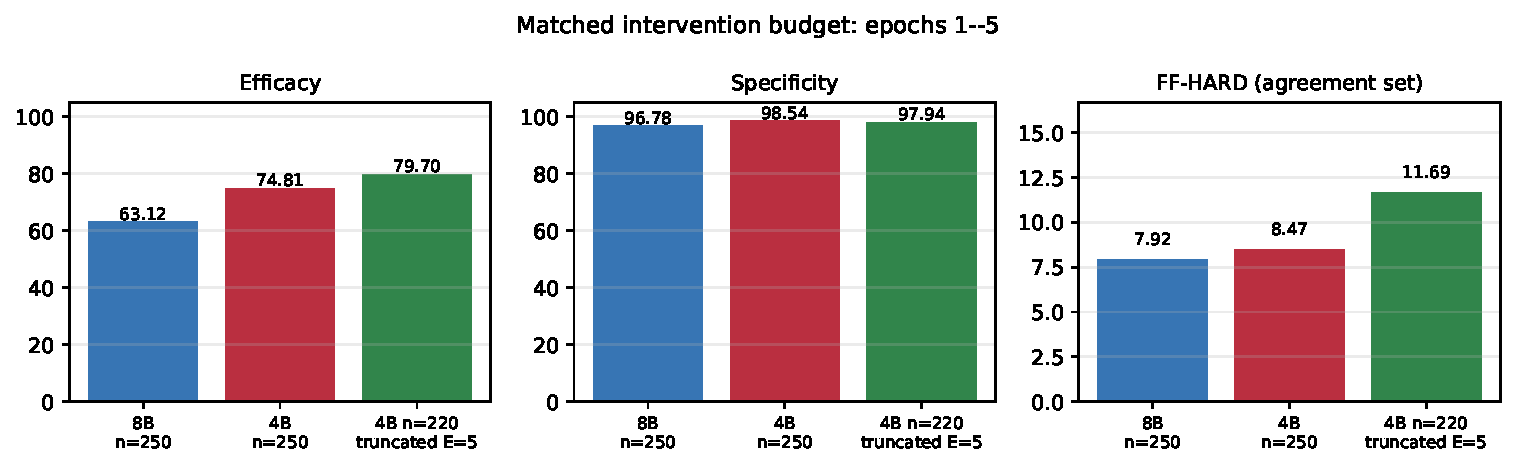
\includegraphics[width=\textwidth]{standard_five_epoch_comparison.pdf}
\caption{统一使用前 5 个 unlearning epoch 时的比较。绿色柱为
\(n=220,E=10\) 运行截取至 epoch 5 的辅助点，并非与两组 \(n=250\)
完全相同的模型规模对照。}
\label{fig:standard}
\end{figure}

两种模型的 \(n=250\) 目标题 ID 完全重合，但各模型生成的 CoT 及切分步骤
并不相同。进一步仅保留两者都满足论文初始预测一致条件的 158 道题，
可以减少可比子集不同造成的偏差。

\begin{table}[H]
\centering
\small
\caption{两种模型在共同初始可比题目上的比较。CoT 文本由各自模型生成，故不是相同步骤的逐步配对。}
\label{tab:paired}
\begin{tabular}{lrrrr}
\toprule
模型 & 共同可比题 & FF-HARD(1--5) & FF-HARD(E5) & Max FF-SOFT \\
\midrule
Qwen3-8B & 158 & 6.96\% & 6.33\% & 6.58 \\
Qwen3-4B & 158 & 7.59\% & 6.96\% & 6.58 \\
\bottomrule
\end{tabular}
\end{table}


共同可比题上，4B 的 1--5 epoch FF-HARD 仅比 8B 高 0.63 点，
Max FF-SOFT 近乎相同。这再次提示：本次 4B/8B 的主要显著差异在
干预有效性 Eff，而不是有力的忠实度排序结论。

\section{重点分析：4B 十轮扩展干预}
表~\ref{tab:endpoint} 使用每份文件的最终 checkpoint，因此能复现既有
8B 摘要中的 endpoint 数值（Eff \(=71.50\)，Spec \(=96.84\)，全量
FF-HARD \(=9.13\%\)）。该表也使 \(n=220\) 的十轮终点不会被悄悄当作
五轮结果。

\begin{table}[H]
\centering
\small
\caption{各结果文件最终 checkpoint 的 endpoint 汇总；此口径与既有 8B 摘要的最终态统计一致。}
\label{tab:endpoint}
\begin{tabular}{lrrrrrr}
\toprule
实验 & 终点 E & Eff & Spec & FF-HARD(all) & FF-HARD(agree) & Mean soft \\
\midrule
Qwen3-8B ($n=250$) & 5 & 71.50 & 96.84 & 9.13\% & 6.93\% & 3.36 \\
Qwen3-4B ($n=250$) & 5 & 81.50 & 98.56 & 9.57\% & 7.91\% & 4.38 \\
Qwen3-4B ($n=220$) & 10 & 90.25 & 98.04 & 12.00\% & 10.39\% & 6.08 \\
\bottomrule
\end{tabular}
\end{table}


对同一个 \(4B,n=220\) 运行进行内部比较，epoch 5 到 epoch 10 的变化为：
\[
\begin{array}{lrrrrr}
 & \mathrm{Eff} & \mathrm{Spec} & \mathrm{FF\mbox{-}HARD(all)}
 & \mathrm{FF\mbox{-}HARD(agree)} & \mathrm{Mean\ soft}\\
\text{E5} & 88.99 & 97.84 & 11.00\% & 9.74\% & 5.42\\
\text{E10} & 90.25 & 98.04 & 12.00\% & 10.39\% & 6.08\\
\Delta & +1.26 & +0.20 & +1.00 & +0.65 & +0.66
\end{array}
\]
延长更新确实进一步降低目标步骤概率并增加答案变化证据；不过收益在约
epoch 6 后已趋于饱和，且 FF-HARD 会随 epoch 小幅波动（例如全量终点指标
在 epoch 6--7 达到 12.50\%，epoch 10 为 12.00\%）。这正是报告完整轨迹
而非只挑选最高终点的原因。

\begin{figure}[H]
\centering
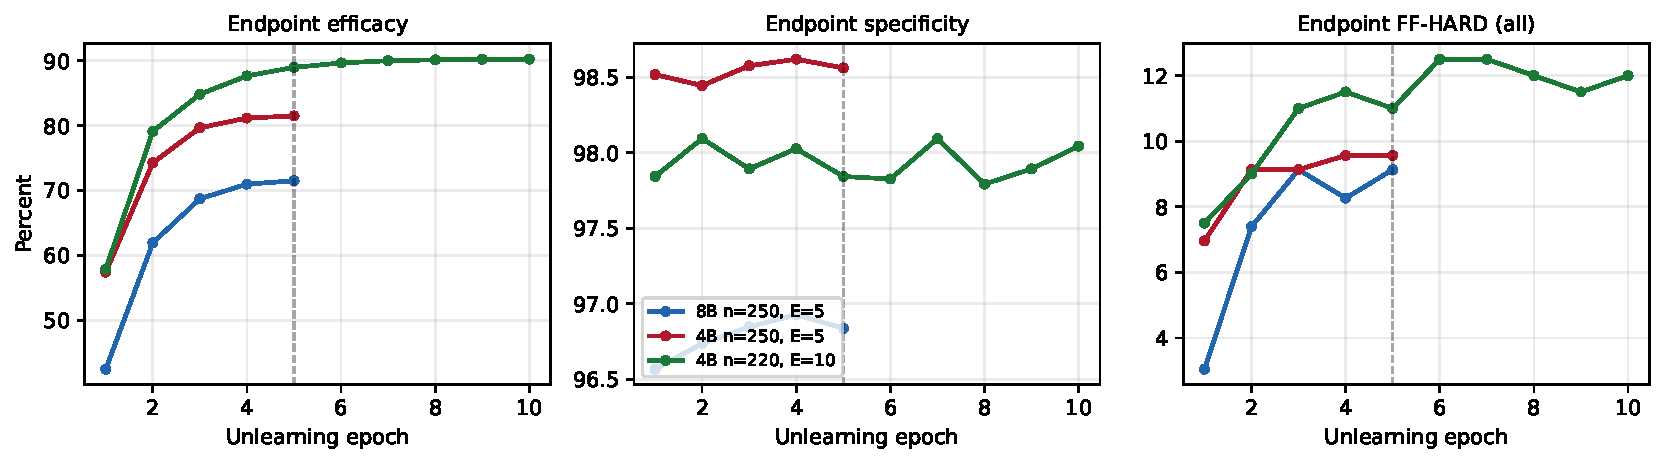
\includegraphics[width=\textwidth]{epoch_trajectories.pdf}
\caption{每个 checkpoint 的终点式指标轨迹。虚线表示原论文与两组标准运行
的 epoch 5 预算；绿色曲线右侧部分只属于 4B 扩展干预。}
\label{fig:epochs}
\end{figure}

\begin{figure}[H]
\centering
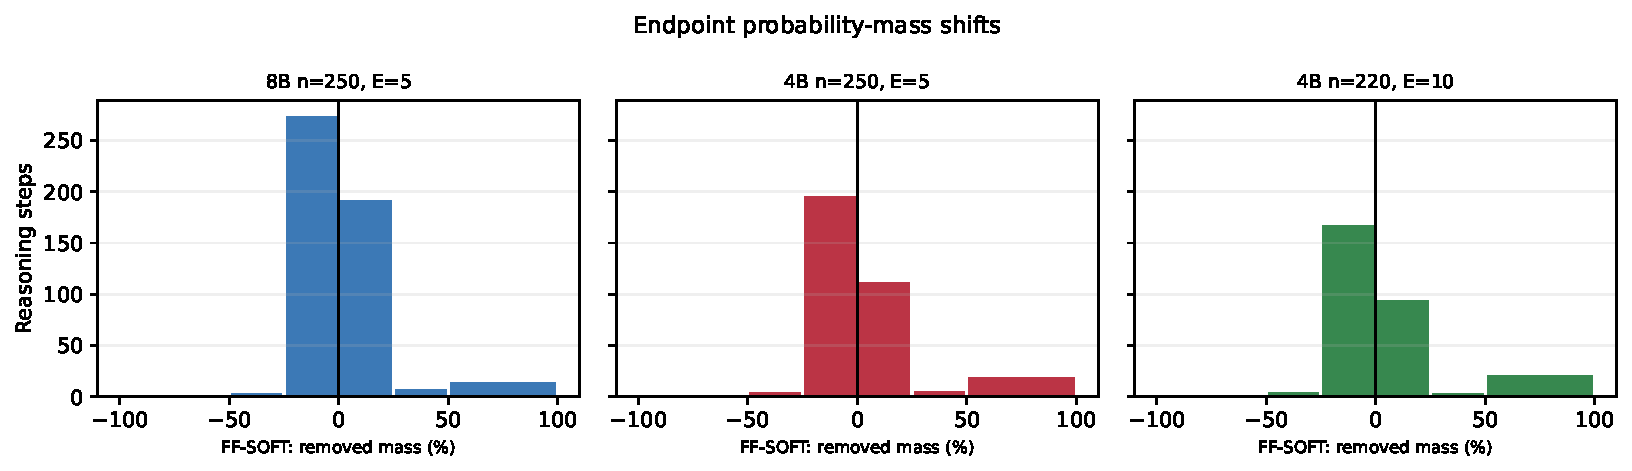
\includegraphics[width=\textwidth]{soft_shift_histograms.pdf}
\caption{各文件最终 checkpoint 的步骤级 FF-SOFT 分布。十轮组显示出更多
向右侧（从初始答案移出概率质量）的步骤，但该变化同时受样本集合和 epoch
预算影响。}
\label{fig:soft}
\end{figure}

\section{结论与限制}
本次 C-Eval 中文复现提供了三点结论。第一，三份输出均完成并具备高
specificity（各比较口径约为 96.8--98.6），因而答案翻转不是明显的整体
模型破坏所致。第二，在相同 \(n=250,E=5\) 配置下，Qwen3-4B 的目标步骤
更容易被 NPO+KL 压低，但其 FF-HARD 仅略高于 Qwen3-8B；不能据此宣称
小模型的 CoT 显著更忠实。第三，也是本报告最重要的配置辨析：
\(n=220\) 的 4B 结果实施了 10 个 epoch，延长干预确实提升 Eff、软变化和
硬翻转率；该组应视作 epoch 强度扩展实验，不能直接并入标准模型排名。

本分析仍有局限：它只覆盖 C-Eval 一个中文题库与单个学习率；没有运行原论文
用于宽泛能力保持控制的 MMLU ``Gen'' 评估；中文实现禁用了原文的英语
content-word POS 过滤；两个模型生成的 CoT 步骤不同，因此共同题目的比较也
不是同一推理文本上的严格配对因果实验。这些限制不影响三份输出的内部统计，
但限制了与原论文绝对数值以及模型规模因果效应的直接外推。

\section*{参考文献}
\begin{enumerate}
  \item Martin Tutek, et al. \textit{Measuring Chain of Thought Faithfulness
  by Unlearning Reasoning Steps}. EMNLP 2025.
  \url{https://aclanthology.org/2025.emnlp-main.504/}
  \item C-Eval: A Multi-Level Multi-Discipline Chinese Evaluation Suite for
  Foundation Models. \url{https://cevalbenchmark.com/}
\end{enumerate}

\end{document}
